\documentclass[10pt]{article}
\usepackage{tikz}
\usetikzlibrary{shapes.misc}
\usepackage[margin=0cm]{geometry}
\pagestyle{empty}
\tikzstyle{every node}=[cross out, draw, red]

\begin{document}

\vspace*{\fill}
\begin{center}
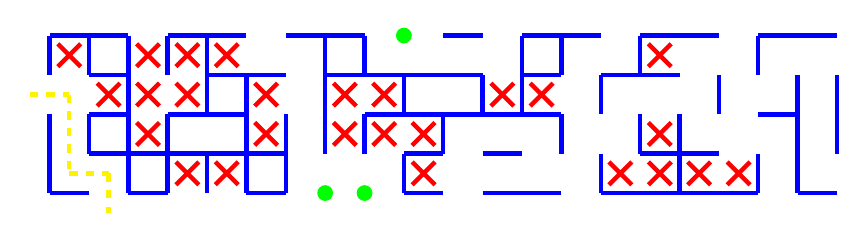
\begin{tikzpicture}[x=0.5cm, y=-0.5cm, ultra thick, blue]
% Walls
    \draw (0,0) -- (2,0);
    \draw (3,0) -- (5,0);
    \draw (6,0) -- (8,0);
    \draw (10,0) -- (11,0);
    \draw (12,0) -- (14,0);
    \draw (15,0) -- (17,0);
    \draw (18,0) -- (20,0);
    \draw (1,1) -- (2,1);
    \draw (4,1) -- (6,1);
    \draw (7,1) -- (11,1);
    \draw (12,1) -- (13,1);
    \draw (14,1) -- (16,1);
    \draw (1,2) -- (2,2);
    \draw (3,2) -- (5,2);
    \draw (8,2) -- (13,2);
    \draw (18,2) -- (19,2);
    \draw (1,3) -- (6,3);
    \draw (9,3) -- (10,3);
    \draw (11,3) -- (12,3);
    \draw (15,3) -- (17,3);
    \draw (0,4) -- (1,4);
    \draw (2,4) -- (3,4);
    \draw (5,4) -- (6,4);
    \draw (9,4) -- (10,4);
    \draw (11,4) -- (13,4);
    \draw (14,4) -- (18,4);
    \draw (19,4) -- (20,4);
    \draw (0,0) -- (0,1);
    \draw (0,2) -- (0,4);
    \draw (1,0) -- (1,1);
    \draw (1,2) -- (1,3);
    \draw (2,0) -- (2,4);
    \draw (3,0) -- (3,1);
    \draw (3,2) -- (3,4);
    \draw (4,0) -- (4,2);
    \draw (4,3) -- (4,4);
    \draw (5,1) -- (5,4);
    \draw (6,2) -- (6,4);
    \draw (7,0) -- (7,3);
    \draw (8,0) -- (8,1);
    \draw (8,2) -- (8,3);
    \draw (9,1) -- (9,2);
    \draw (9,3) -- (9,4);
    \draw (10,2) -- (10,3);
    \draw (11,1) -- (11,2);
    \draw (12,0) -- (12,2);
    \draw (13,0) -- (13,1);
    \draw (13,2) -- (13,3);
    \draw (14,1) -- (14,2);
    \draw (14,3) -- (14,4);
    \draw (15,0) -- (15,1);
    \draw (15,2) -- (15,3);
    \draw (16,2) -- (16,4);
    \draw (17,1) -- (17,2);
    \draw (18,0) -- (18,1);
    \draw (18,3) -- (18,4);
    \draw (19,1) -- (19,4);
    \draw (20,1) -- (20,3);
% Pillars
    \fill[green] (9,0) circle(0.2);
    \fill[green] (7,4) circle(0.2);
    \fill[green] (8,4) circle(0.2);
% Inner points in accessible cul-de-sacs
    \node at (0.5,0.5) {};
    \node at (2.5,0.5) {};
    \node at (3.5,0.5) {};
    \node at (4.5,0.5) {};
    \node at (15.5,0.5) {};
    \node at (1.5,1.5) {};
    \node at (2.5,1.5) {};
    \node at (3.5,1.5) {};
    \node at (5.5,1.5) {};
    \node at (7.5,1.5) {};
    \node at (8.5,1.5) {};
    \node at (11.5,1.5) {};
    \node at (12.5,1.5) {};
    \node at (2.5,2.5) {};
    \node at (5.5,2.5) {};
    \node at (7.5,2.5) {};
    \node at (8.5,2.5) {};
    \node at (9.5,2.5) {};
    \node at (15.5,2.5) {};
    \node at (3.5,3.5) {};
    \node at (4.5,3.5) {};
    \node at (9.5,3.5) {};
    \node at (14.5,3.5) {};
    \node at (15.5,3.5) {};
    \node at (16.5,3.5) {};
    \node at (17.5,3.5) {};
% Entry-exit paths without intersections
    \draw[dashed, yellow] (-0.5,1.5) -- (0.5,1.5);
    \draw[dashed, yellow] (0.5,3.5) -- (1.5,3.5);
    \draw[dashed, yellow] (0.5,1.5) -- (0.5,3.5);
    \draw[dashed, yellow] (1.5,3.5) -- (1.5,4.5);
\end{tikzpicture}
\end{center}
\vspace*{\fill}

\end{document}
